\section{Held-Out Safety-Gym A1--A2 Substep Audit}
\label{sec:sg-contract-v1}

We tested whether the MuJoCo interface used by the paired Safety-Gym study
accepts the plant contract assumed by the conditional safety theorem.  The
protocol was frozen before execution (SHA-256
\texttt{4eaecac9c0c31efc}\allowbreak
\texttt{b97fde888fb85949}\allowbreak
\texttt{74a21fe54f7f23cd}\allowbreak
\texttt{0e5205198061cfe2}).
It covers both training modes, all three tasks, and all five checkpoints per
cell: 30 checkpoint cells, 20 fresh reset seeds per checkpoint, 600 episodes,
and 516,966 held actions.  The held-out seeds 271000--271019 are disjoint from
all strict and ABER-LR paired evaluation schedules.  No actor training, model fitting,
threshold search, or post-hoc tolerance selection was performed.

For every 20-ms held action, the collector records all ten actual MuJoCo
substeps at 2~ms resolution.  The frozen primary stratum requires a certified
state at the beginning of the hold and no non-ground contact in any substep.
An independent raw-trace auditor checks file/checkpoint provenance, action
clipping, substep count and timing, support, and three zero-violation gates:
the A1 next-speed and held-path bounds and the A2 recovery inequality for the
executed $(0,0)$ action.  All integrity and support gates pass, but each
contract gate fails (Table~\ref{tab:sg-contract-v1}).

\begin{table}[t]
\centering
\small
\setlength{\tabcolsep}{3.0pt}
\begin{tabular}{lrrrr}
\toprule
Gate & Support & Violations & Rate & Maximum\\
\midrule
A1 next speed & 231,236 & 28,041 & 12.13\% & 0.10301 m/s\\
A1 held path  & 231,236 &  3,567 &  1.54\% & 0.001300 m\\
A2 recovery   &  39,290 & 35,517 & 90.40\% & 0.013107 m\\
\bottomrule
\end{tabular}
\caption{Frozen primary-stratum result.  ``Maximum'' is the maximum signed
contract residual; the frozen numerical tolerance is $10^{-9}$.}
\label{tab:sg-contract-v1}
\end{table}

\begin{figure}[t]
\centering
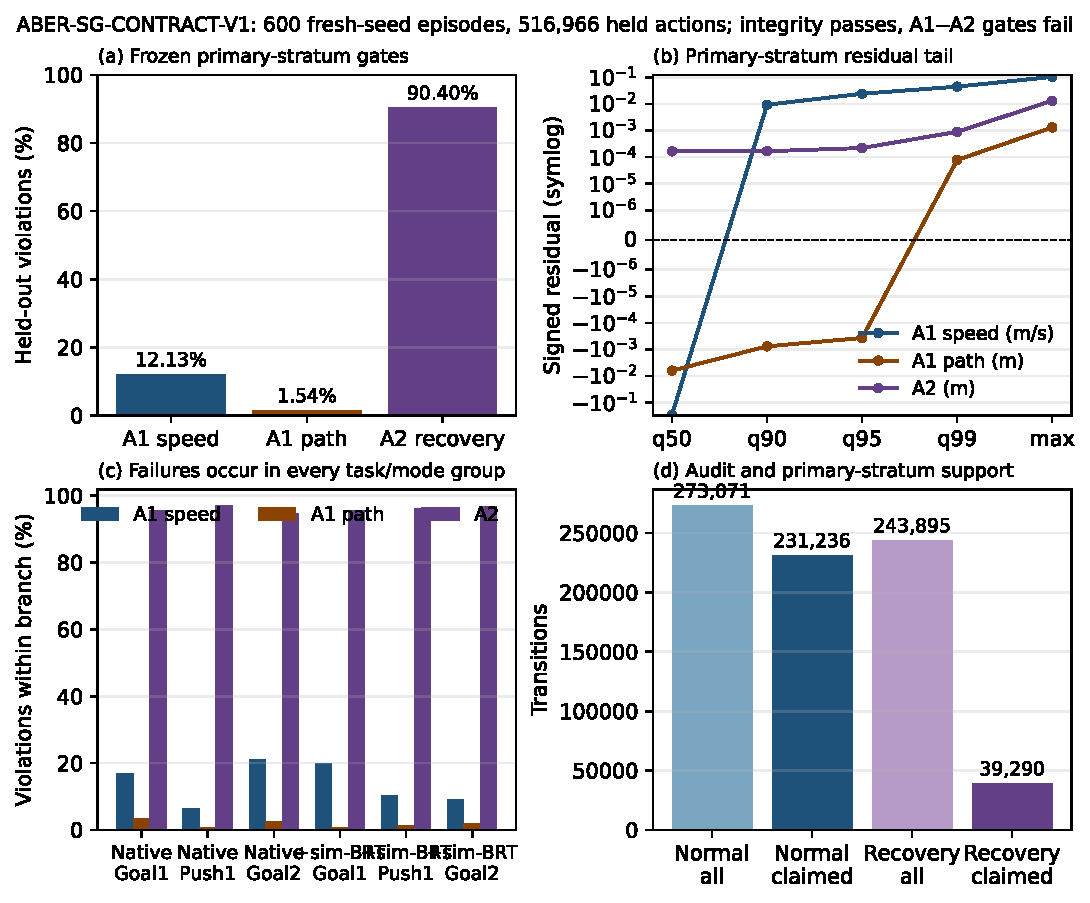
\includegraphics[width=\linewidth]{../figures/supplement/aber_safetygym_contract_v1.pdf}
\caption{The held-out contract audit.  Failures remain after excluding every
hold with non-ground contact and occur in every task/training-mode group.}
\label{fig:sg-contract-v1}
\end{figure}

The V1 decision is therefore a \emph{no-go} for connecting the current
$a_b=0.9$, $v_{\max}=1.5$, $\Delta t=0.02$ Safety-Gym experiments to the
unmodified A1--A2 envelope.  This is not a failure of the conditional theorem
or a retraction of the paired empirical collision comparison.  It establishes
the sharper boundary: the model-matched benchmark tests the theorem under its
assumptions, whereas the Safety-Gym matrix remains empirical and cannot be
called theorem validation.  In particular, current Safety-Gym data do not
certify $(0,0)$ as the required recovery and do not yet justify MuJoCo
ABER-FP directional-tube confirmation.

The complete frozen protocol, aggregate audit, raw gzip traces, collector,
substep instrumentation, independent auditor, plotting script, and focused
tests are included in the reproducibility materials.  A successor contract
must be separately named and pre-frozen.  It may restrict the accepted
operating region or use a conservative measured envelope conditioned on
starting speed, executed forward/turn commands, actuator mode, and contact
topology; it must not reinterpret V1 or tune a constant to these held-out
failures.
